\documentclass[aspectratio=169,11pt]{beamer}
\usepackage[utf8]{inputenc}
\usepackage[brazil]{babel}
\usepackage[T1]{fontenc}
\usepackage{graphicx,booktabs}
\usepackage{xcolor}

\definecolor{navy}{HTML}{26215C}
\definecolor{rxpurple}{HTML}{534AB7}
\definecolor{rxteal}{HTML}{1D9E75}

\usetheme{default}
\setbeamertemplate{navigation symbols}{}
\setbeamertemplate{footline}[frame number]
\setbeamercolor{frametitle}{fg=navy}
\setbeamercolor{title}{fg=navy}
\setbeamercolor{structure}{fg=rxpurple}
\setbeamercolor{alerted text}{fg=rxteal}
\setbeamerfont{frametitle}{series=\bfseries}
\setbeamerfont{title}{series=\bfseries}

\title{xR --- Recuperação Esperada sob Pressão}
\subtitle{Um modelo logístico calibrado com alvo espacialmente restrito}
\author{Abraão C. Gomes \and Giovanni Paes \and Rafael Lúcio}
\institute{UFRJ --- COE609}
\date{SBPO 2026}

\begin{document}

% ---- Título ----
{\setbeamertemplate{footline}{}\begin{frame}\titlepage\end{frame}}

% ---- 1. Introdução / objetivo ----
\begin{frame}{Introdução \& objetivo}
  \begin{columns}[T]
    \begin{column}{0.56\textwidth}
      {\large ``\textit{O jogador deveria perder a bola sob pressão?}''}
      \vspace{4mm}
      \begin{itemize}
        \item \emph{Pressing} é pilar tático do futebol de elite.
        \item Modelos da literatura estacionam em AUC $\approx$\,0,60 --- \alert{sem explicar o porquê}.
        \item \emph{Ratings} individuais são apresentados \alert{sem auditoria}.
      \end{itemize}
    \end{column}
    \begin{column}{0.42\textwidth}
      \begin{block}{Proposta}
        \textbf{xR} = probabilidade \emph{calibrada} de a equipe que pressiona \textbf{recuperar a bola}
        \\(do lado do portador: risco de \emph{perder} a posse).
      \end{block}
    \end{column}
  \end{columns}
\end{frame}

% ---- 2. Dados usados ----
\begin{frame}{Dados usados}
  \centering
  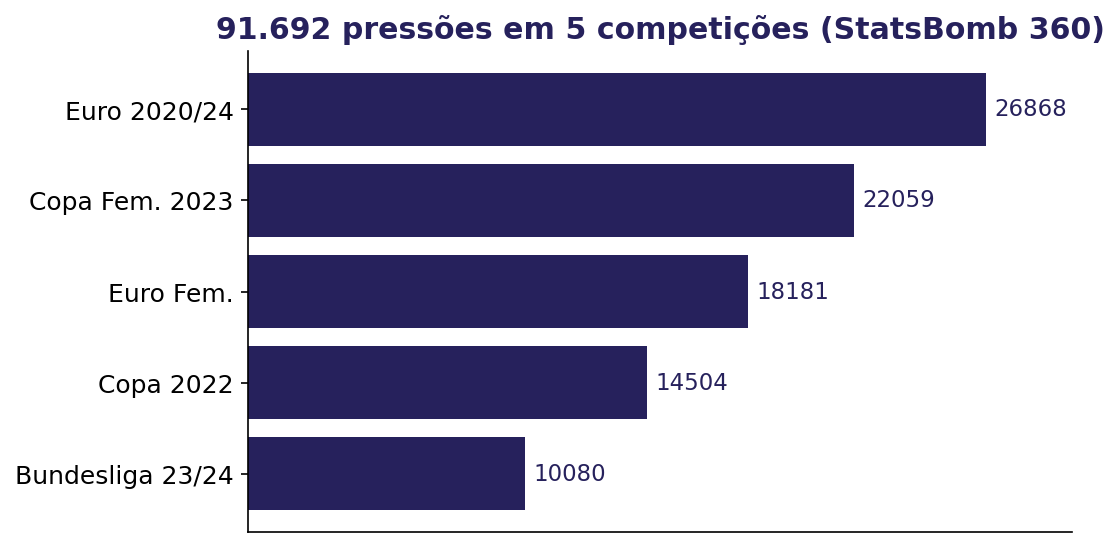
\includegraphics[height=0.66\textheight]{figs/slide_competitions.png}

  {\small StatsBomb 360 --- \emph{freeze frame} por evento (posições visíveis). Unidade = cada pressão.}
\end{frame}

% ---- 3. Modelo inicial ----
\begin{frame}{Modelo inicial}
  \centering
  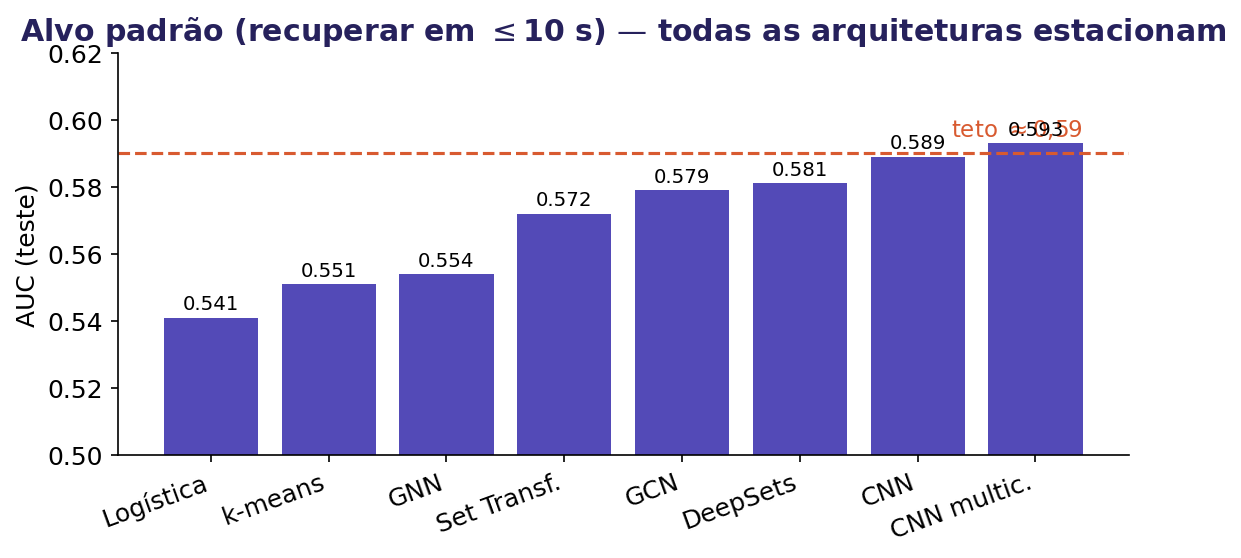
\includegraphics[height=0.66\textheight]{figs/slide_plateau.png}

  \alert{A arquitetura não move o teto} --- regras, $k$-means, GNN, CNN e Set Transformer todos $\approx$\,0,59.
\end{frame}

% ---- 4. Estudo de contra-pressão ----
\begin{frame}{Estudo de contrapressão}
  \centering
  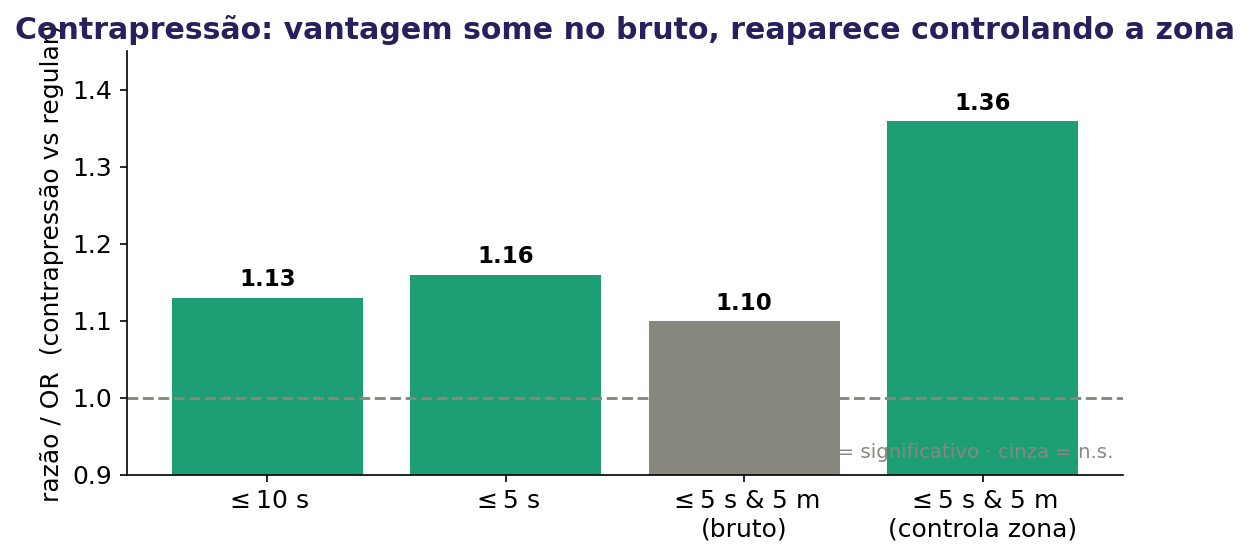
\includegraphics[height=0.62\textheight]{figs/slide_counterpress.png}

  {\small Clara no alvo permissivo; no estrito \alert{some na comparação bruta} (confundimento por zona) e
  \alert{reaparece ao controlar a zona} (OR 1,36).}
\end{frame}

% ---- 5. Estudo de triggers ----
\begin{frame}{Estudo de gatilhos (\emph{triggers})}
  \centering
  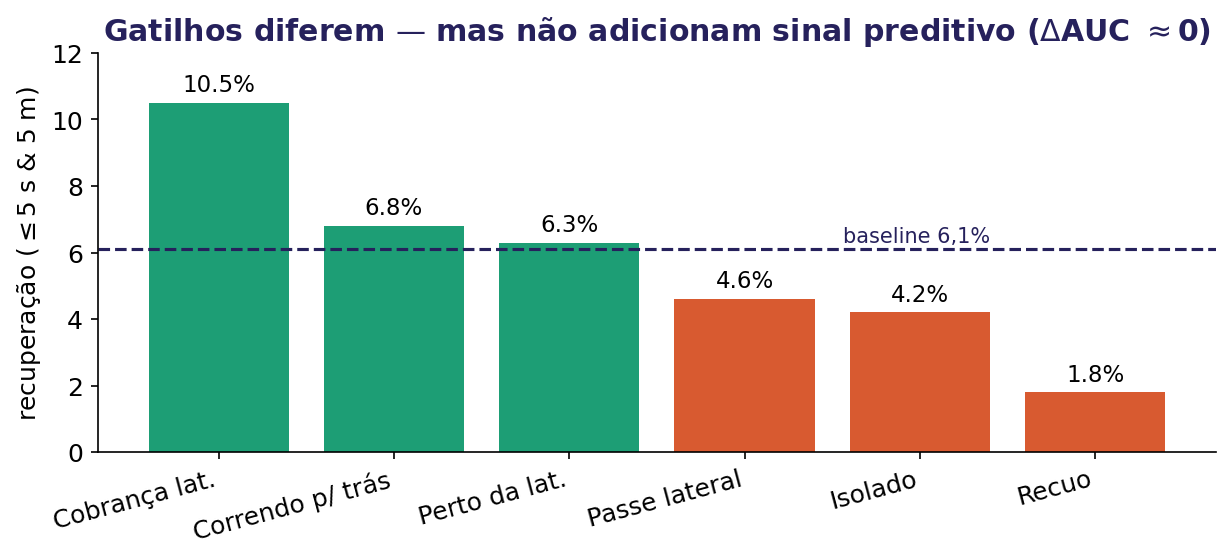
\includegraphics[height=0.62\textheight]{figs/slide_triggers.png}

  {\small Os gatilhos \emph{descrevem} bem (recuo 0,30$\times$ \dots cobrança 1,73$\times$), mas
  \alert{não adicionam sinal preditivo} ao modelo ($\Delta$AUC $\approx$\,0).}
\end{frame}

% ---- 6. Estudo de impacto da geometria ----
\begin{frame}{Impacto da geometria --- relação dose-resposta}
  \begin{columns}[T]
    \begin{column}{0.56\textwidth}
      \centering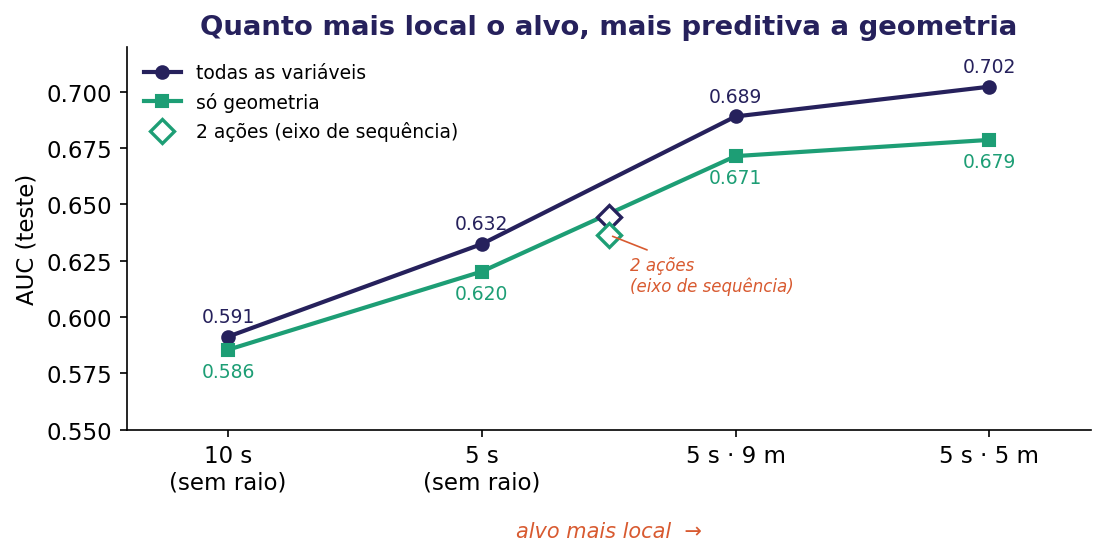
\includegraphics[width=\linewidth]{figs/fig_ladder.png}
    \end{column}
    \begin{column}{0.44\textwidth}
      \small
      \begin{itemize}
        \item Alvo com raio: \alert{atribuído ao exPress}; nós \alert{explicamos por quê}.
        \item Quanto mais \emph{local} o alvo, mais preditiva a geometria.
        \item Mecanismo: \alert{76\%} das recuperações em $\leq$10\,s são ruído causal (mediana 13\,m).
        \item Controle de \emph{base rate} + \emph{bootstrap}: ganho \alert{real}, não artefato.
      \end{itemize}
    \end{column}
  \end{columns}
\end{frame}

% ---- 7b. Base rate não explica o ganho ----
\begin{frame}{O base rate explica o ganho? \alert{Não}}
  \begin{columns}[T]
    \begin{column}{0.54\textwidth}
      \centering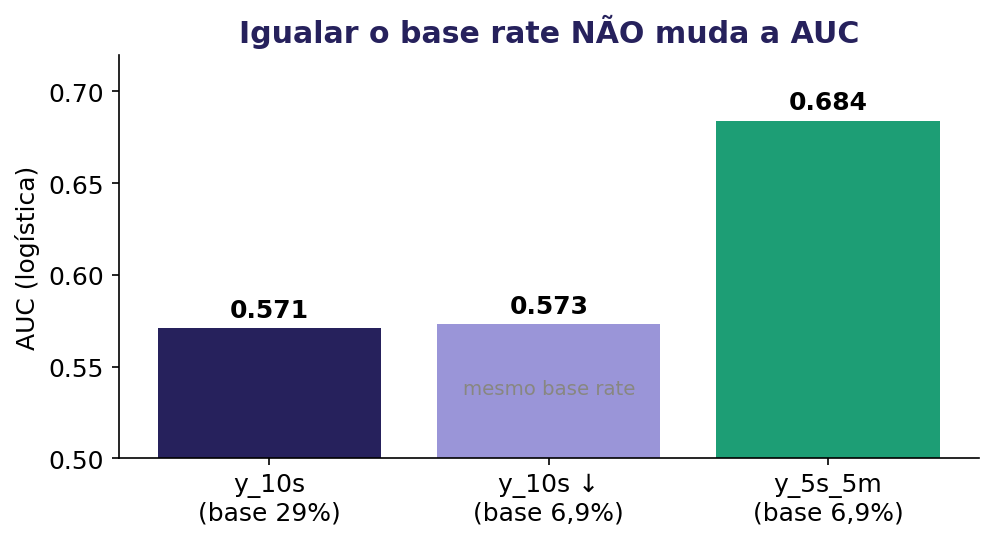
\includegraphics[width=\linewidth]{figs/slide_baserate.png}
    \end{column}
    \begin{column}{0.46\textwidth}
      \small
      \begin{itemize}
        \item \textbf{ROC-AUC é invariante à prevalência} (estatística de ranqueamento).
        \item \textbf{Controle:} rebaixar o alvo permissivo a 6,9\% (\emph{downsample}, 25$\times$) $\to$ AUC \alert{0,573} ($=$0,571 cheia).
        \item \emph{Gap} estrito$-$permissivo $=$ \alert{$+0{,}113$}; IC95\% \emph{bootstrap} $[0{,}100;\,0{,}124]$.
      \end{itemize}
    \end{column}
  \end{columns}
\end{frame}

% ---- 7c. Calibração ----
\begin{frame}{Calibração --- habilita o uso agregado}
  \begin{columns}[T]
    \begin{column}{0.5\textwidth}
      \centering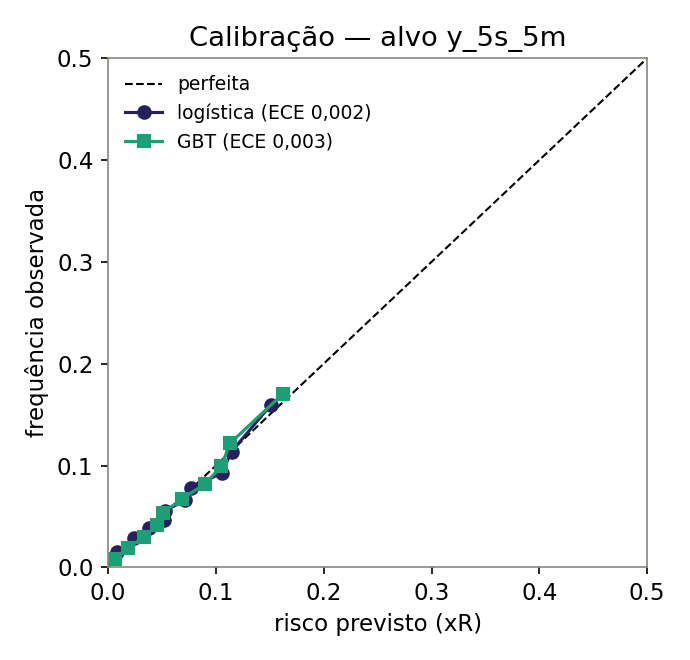
\includegraphics[width=\linewidth]{figs/fig_calibration.png}
    \end{column}
    \begin{column}{0.5\textwidth}
      \small ``20\% previsto $\Rightarrow$ $\approx$20\% observado''.\\[1mm]
      \textbf{ECE} $=$ erro médio de calibração; \textbf{Brier} $=$ erro quadrático da probabilidade.
      \begin{center}
        \begin{tabular}{lcc}
          \toprule
          Modelo & ECE & Brier \\
          \midrule
          Logística & \textbf{0,002} & 0,063 \\
          GBT & 0,003 & 0,062 \\
          \bottomrule
        \end{tabular}
      \end{center}
      \alert{Bem calibrado} $\Rightarrow$ legítimo em \textbf{agregado} (linhagem do xG).
    \end{column}
  \end{columns}
\end{frame}

% ---- 7d. Confiabilidade de ratings individuais ----
\begin{frame}{Rating individual de jogador --- \alert{não confiável}}
  \centering
  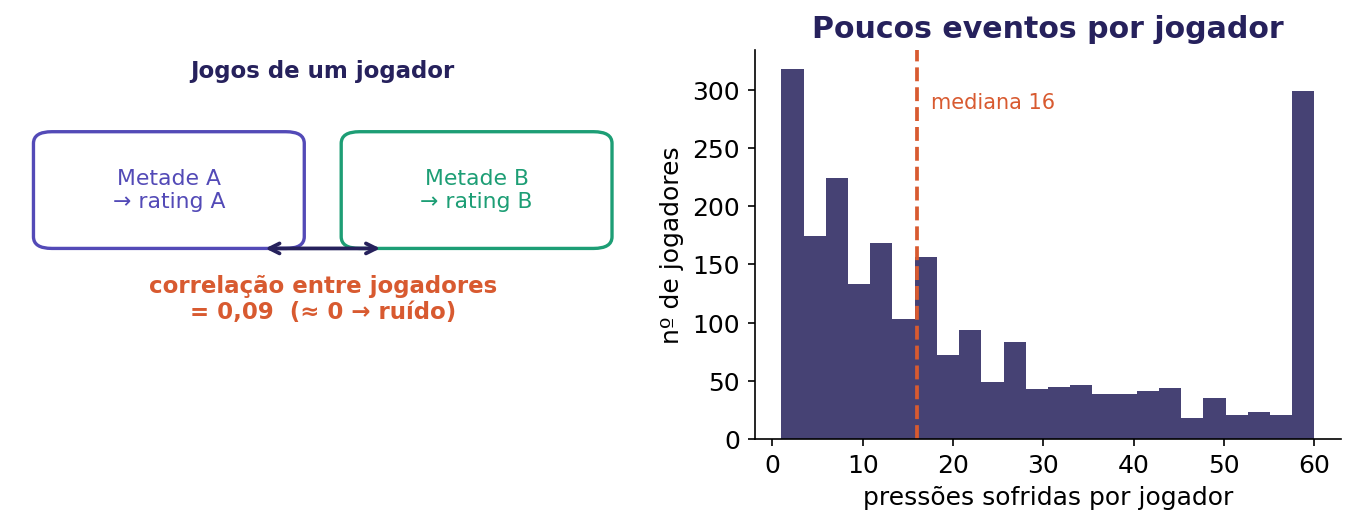
\includegraphics[height=0.56\textheight]{figs/slide_reliability.png}

  {\small \textbf{Split-half}: divide os jogos de cada jogador em 2, calcula o rating em cada metade e correlaciona entre jogadores. Deu \alert{0,09} (usável pede $\geq$0,5) --- causa: mediana de \alert{16 pressões/jogador}.}
\end{frame}

% ---- 7. Conclusões ----
\begin{frame}{Conclusões}
  \begin{enumerate}
    \item[\textcolor{rxpurple}{\textbf{1.}}] \textbf{Mecanismo (dose-resposta).} Quanto mais local o alvo, mais informativa
    a geometria (só-geometria 0,59$\to$\alert{0,68}); \alert{76\%} das recuperações em $\leq$10\,s são ruído causal.
    O alvo é da literatura --- nós explicamos \emph{por quê}.
    \vspace{2mm}
    \item[\textcolor{rxpurple}{\textbf{2.}}] \textbf{Modelo leve e calibrado.} Uma regressão logística (ECE 0,003) iguala
    GNN/CNN e é interpretável.
    \vspace{2mm}
    \item[\textcolor{rxpurple}{\textbf{3.}}] \textbf{Escopo honesto.} \emph{Rating} individual de jogador tem confiabilidade
    $\approx$\,\alert{0,09} --- \textbf{não} serve para veredito individual.
  \end{enumerate}
\end{frame}

% ---- 8. Aplicação prática ----
\begin{frame}{Aplicação prática}
  \centering
  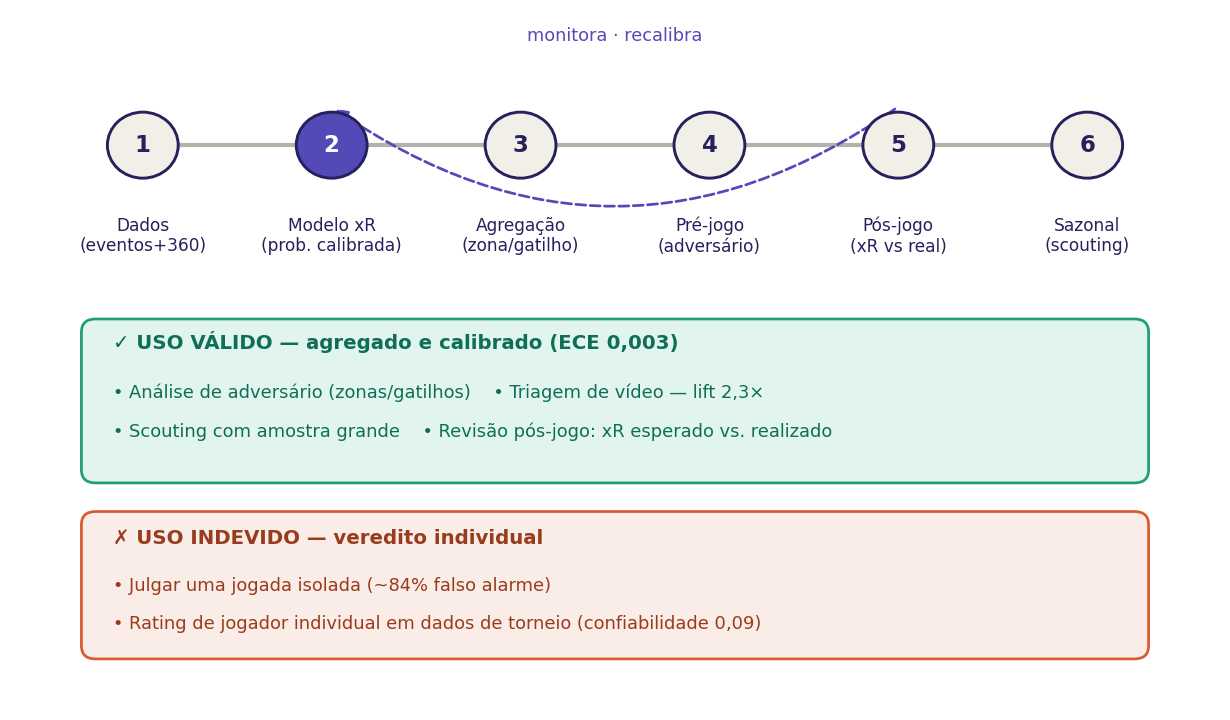
\includegraphics[height=0.78\textheight]{figs/fig_flow.png}
\end{frame}

% ---- 9. Exemplo / casos de uso ----
\begin{frame}{Exemplo / caso de uso --- revisão pós-jogo}
  \centering
  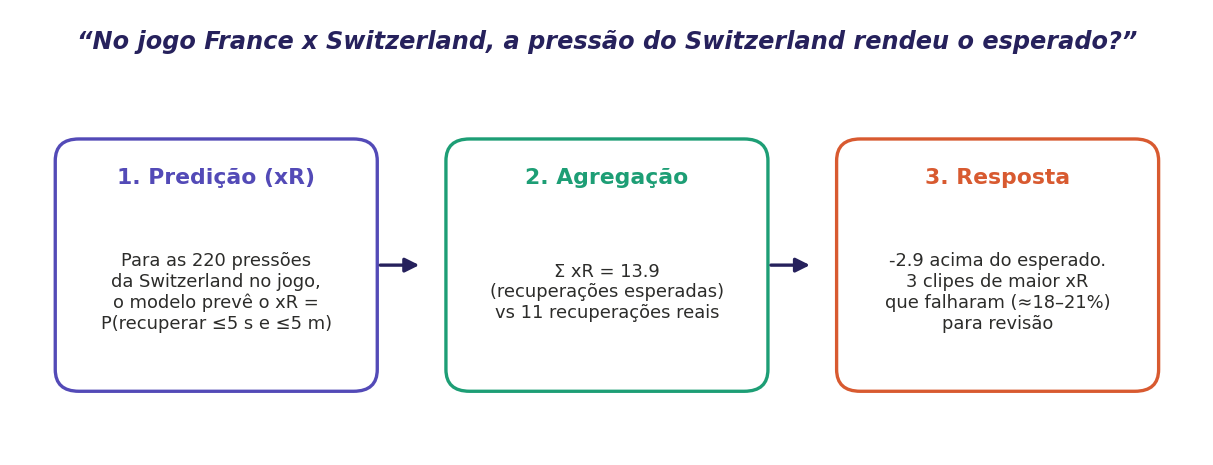
\includegraphics[width=0.96\textwidth]{figs/fig_usecase.png}

  {\small Pergunta da comissão $\to$ predição (xR por pressão) $\to$ resposta.}
\end{frame}

\begin{frame}{Caso de uso 1 --- análise de adversário (pré-jogo)}
  \small
  \textbf{Pergunta:} ``Vamos enfrentar a Itália --- em que zona a nossa pressão tem mais chance de recuperar a bola?''

  \vspace{1mm}
  \textbf{Como:} pega as pressões \emph{sofridas} pela Itália (Itália em posse); o modelo dá o xR de
  cada uma (\,xR $=$ chance de a Itália \alert{perder} a bola\,); agrega-se por terço do campo, na
  ótica da Itália (que ataca à direita).

  \vspace{1mm}
  \textbf{Resultado:} xR médio bem maior no \alert{terço defensivo da Itália} (perto do gol dela),
  \alert{8,4\%}, do que no terço de ataque dela, 3,8\%.

  \vspace{1mm}
  \textbf{Resposta:} a Itália perde mais a bola sob pressão \alert{alta} (no próprio campo de defesa)
  --- é onde priorizar o \emph{gegenpressing}.
\end{frame}

\begin{frame}{Caso de uso 2 --- triagem de vídeo}
  \small
  \textbf{Pergunta:} ``Pouco tempo de análise --- quais pressões revisar primeiro?''

  \vspace{1mm}
  \textbf{Como:} \emph{ordene} todas as pressões pela xR (maior $\to$ menor) e revise só o
  \textbf{topo}. Como xR alto recupera mais, as \alert{recuperações} (o time que pressiona ganha a
  bola) se concentram no topo.
  \begin{center}
    \begin{tabular}{ccc}
      \toprule
      Vídeo revisado & Recuperações & \emph{lift} \\
      (\% de maior xR) & encontradas & (vs.\ acaso) \\
      \midrule
      5\%  & 17\% & 3,4$\times$ \\
      10\% & \alert{28\%} & \alert{2,9$\times$} \\
      20\% & 44\% & 2,2$\times$ \\
      \bottomrule
    \end{tabular}
  \end{center}
  {\footnotesize \emph{lift} $=$ recuperações $\div$ \% revisado ($28\%\div10\%=2{,}9\times$ o acaso).
  \textbf{Revisando 10\% do vídeo, acha-se 28\% de todas as recuperações.}}
\end{frame}

\end{document}
